\documentclass[letterpaper,11pt,onecolumn]{article}
\usepackage[utf8]{inputenc}
\usepackage{fontenc}
\usepackage{amsmath}
\usepackage{graphicx}
\usepackage[top=1.85cm, left=2cm, bottom=2cm, right=2cm]{geometry}
\setlength{\parindent}{0cm}
\usepackage{booktabs}
\usepackage{cite}
\usepackage{enumitem}
\usepackage{hyperref}
\usepackage{comment}
\usepackage{multicol}
\usepackage[version=4]{mhchem}
\usepackage{lipsum}
\usepackage{bm}


\title{Schwartzschild Geometry: Metric, Geodesics and Black Holes}
\author{ Alejandro Gómez$^1$, Juan E. Bedoya$^1$, Nicolle Tello$^1$, Stiven Londoño$^1$ \\ $^1$\textit{Departamento de Física, Universidad del Valle} }
\date{\today}

\begin{document}

\maketitle

\begin{abstract}
    \lipsum[1]
\end{abstract}


\section{Introduction}\label{intro}

\lipsum[1]

\begin{figure}[h!]
    \centering
    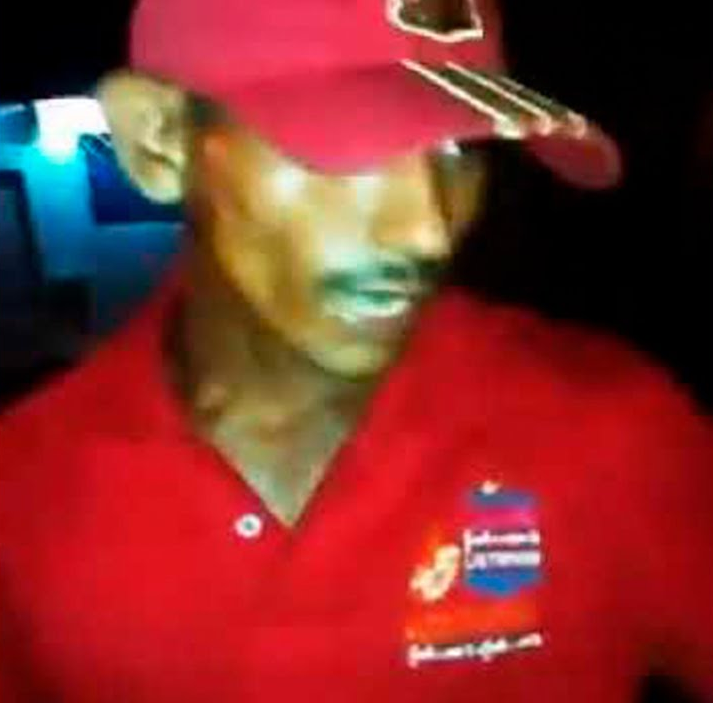
\includegraphics[width=0.3\textwidth]{Report/Images/sample.png}
\end{figure}

\section{Metric}\label{metric}

\lipsum[2]

\begin{equation}
    ds^2 = \cdots
\end{equation}

\section{Geodesics}

\lipsum[2]

\subsection{Massive particles}

\lipsum[3]

\subsection{Massless particles}

\lipsum[3]

\section{Black Holes}

\lipsum[4]

\section{References}



\end{document}